\chapter{การทดสอบระบบ}
การทดสอบการทำงานขอแอนดรอยด์งแอปพลิเคชันระบบกองทุนเงินให้กู้ยืมเพื่อการศึกษา คณะวิทยาศาสตร์ มหาวิทยาลัยอุบลราชธานีและทดสอบการทำงานในส่วนของเว็บไซต์ โดยทำการทดสอบในลักษณะ Black-box Testing \cite{blackbox} หรือ Data-Driven testing ซึ่งเป็นการเทสแบบที่ไม่สนใจโปรเซส (Process) การทำงานภายในของโปรแกรมว่าทำงานอย่างไร แต่จะเน้นไปที่ Input และ Result ที่ได้มากกว่าว่าการทำงานต่าง ๆ ถูกต้องตามความต้องการ (Requirement) หรือไม่ ซึ่งการทดสอบการใช้งานแอนดรอยด์แอปพลิเคชัน และ ความแม่นยำของ Tensorflow Lite ได้ผลดังนี้

	\section{การทดสอบการใช้งานแอนดรอยด์แอปพลิเคชัน}
		\begin{itemize}
					\item{การทดสอบการใช้งานเมนูนำทางของแอนดรอยด์แอปพลิเคชัน}
					การทดสอบเมนูนำทางของแอปพลิเคชันในการนำทางสมาชิก ซึ่งเมนูหลักประกอบด้วย เมนูเข้าสู่ระบบ เมนูแดชบอร์ด เมนูสแกน เมนูเพิ่มอาหาร หน้าจอการดูข้อมูลการบริโภคแบบสัปดาห์  หน้าจอการดูข้อมูลการบริโภคแบบเดือน เมนูตั้งค่า ผลทดสอบดังตารางที่ \ref{tab:ผลการทดสอบเมนูนำทาง}-\ref{tab:การทดสอบหน้าเมนูตั้งค่า}
					\begin{table}[H]
						\caption{ผลการทดสอบเมนูนำทาง}
						\centering	
						\label{tab:ผลการทดสอบเมนูนำทาง}
						\begin{tabular}{ | p{4.5cm} | p{4.5cm} | p{4.5cm} | }
							\hline
							% {\setstretch{1.0} } 
							{\multicolumn{1}{c}{\centering การทำงาน}}  & 
							{\multicolumn{1}{c}{\centering เงื่อนไขการทดสอบ}} & {\multicolumn{1}{c}{\centering ผลการทดสอบ}} \\ \hline
							\setstretch{1.0}{เมนูแดชบอร์ด} 
							& \setstretch{1.0}{กดปุ่มเมนูแดชบอร์ด}
							& \setstretch{1.0}{ระบบแสดงผลหน้าจอแดชบอร์ดพร้อมแถบสำหรับเลื่อนดูข้อมูลการบริโภครูปแบบสัปดาห์และเดือน} \\ \hline
							\setstretch{1.0}{เมนูสแกน} 
							& \setstretch{1.0}{กดปุ่มเมนูสแกน}
							& \setstretch{1.0}{ระแบบแสดงผลหน้าจอสแกนพร้อมกับเปิดกล้อง} \\ \cline{2-3} 
							& \setstretch{1.0}{กดปุ่มย้อนกลับ} 
							& \setstretch{1.0}{ระบบทำการปิดแอปพลิเคชัน} \\ \hline
							\setstretch{1.0}{เมนูเพิ่มอาหาร} 
							& \setstretch{1.0}{กดปุ่มเมนูเพิ่มอาหาร}
							& \setstretch{1.0}{ระแบบแสดงผลหน้าจอเพิ่มอาหารและมีรายการอาหารที่เพิ่มแล้วมาแสดง} \\ \cline{2-3} 
							& \setstretch{1.0}{กดปุ่มย้อนกลับ} 
							& \setstretch{1.0}{ระบบทำการปิดแอปพลิเคชัน} \\ \hline
							\setstretch{1.0}{หน้าจอการดูข้อมูลการบริโภคแบบสัปดาห์} 
							& \setstretch{1.0}{เลื่อนไปแถบข้อมูลการบริโภคแบบสัปดาห์}
							& \setstretch{1.0}{ระบบแสดงรายการข้อมูลการบริโภคของแต่ละสัปดาห์} \\ \cline{2-3} 
							& \setstretch{1.0}{กดปุ่มย้อนกลับ} 
							& \setstretch{1.0}{ระบบทำการปิดแอปพลิเคชัน} \\ \hline
							\setstretch{1.0}{หน้าจอการดูข้อมูลการบริโภคแบบเดือน} 
							& \setstretch{1.0}{เลื่อนไปแถบข้อมูลการบริโภคแบบเดือน}
							& \setstretch{1.0}{ระบบแสดงรายการข้อมูลการบริโภคของแต่ละเดือน} \\ \cline{2-3} 
							& \setstretch{1.0}{กดปุ่มย้อนกลับ} 
							& \setstretch{1.0}{ระบบทำการปิดแอปพลิเคชัน} \\ \hline
							\setstretch{1.0}{เมนูตั้งค่า} 
							& \setstretch{1.0}{กดเมนูตั้งค่า}
							& \setstretch{1.0}{ระบบแสดงเมนูตั้งค่า} \\ \cline{2-3} 
							& \setstretch{1.0}{กดปุ่มย้อนกลับ} 
							& \setstretch{1.0}{ระบบแสดงผลหน้าจอแดชบอร์ดพร้อมแถบสำหรับเลื่อนดูข้อมูลการบริโภครูปแบบสัปดาห์และเดือน} \\ \hline
						\end{tabular}
					\end{table}
						
						\newpage
					\item{การทดสอบหน้าแดชบอร์ด}
					ในการแสดงผลหน้าจอรายละเอียดประกาศนั้นจะประกอบไปด้วย Chart สำหรับการดูรายละเอียดการบริโภคพร้อมกับแถบสำหรับดูข้อมูลการบริโภครูปแบบสัปดาห์และเดือน  ผลการทดสอบดังตารางที่ \ref{tab:การทดสอบหน้าแดชบอร์ด}
					\begin{table}[H]
						\caption{ผลการทดสอบหน้าแดชบอร์ด}
						\centering	
						\label{tab:การทดสอบหน้าแดชบอร์ด}
						\begin{tabular}{ | p{4.5cm} | p{4.5cm} | p{4.5cm} | }
							\hline
							% {\setstretch{1.0} } 
							{\multicolumn{1}{c}{\centering การทำงาน}}  & 
							{\multicolumn{1}{c}{\centering เงื่อนไขการทดสอบ}} & {\multicolumn{1}{c}{\centering ผลการทดสอบ}} \\ \hline
							\setstretch{1.0}{หน้าแดชบอร์ด} 
							& \setstretch{1.0}{เลื่อนไปยังแถบ Week}
							& \setstretch{1.0}{ระบบแสดงรายการข้อมูลการบริโภคของแต่ละสัปดาห์} \\ \cline{2-3} 
							& \setstretch{1.0}{เลื่อนไปยังแถบ Month} 
							& \setstretch{1.0}{ระบบแสดงรายการข้อมูลการบริโภคของแต่ละเดือน} \\ \cline{2-3} 
							& \setstretch{1.0}{เลื่อนกลับมายังแถบ Week}} 
							& \setstretch{1.0}{ระบบแสดงรายการข้อมูลการบริโภคของแต่ละสัปดาห์} \\ \cline{2-3} 
							& \setstretch{1.0}{เลื่อนกลับมายังแถบ Day} 
							& \setstretch{1.0}{ระบบแสดง Chart และรายระเอียดการบริโภคของวัน} \\ \hline
						\end{tabular}
					\end{table}
				
					\newpage
					\item{การทดสอบหน้าสแกน}ในการแสดงผลหน้าจอสนทนานั้นจะประกอบไปด้วยกล้องสำหรับทำการถ่ายภาพ ปุ่ม Scan  ผลการทดสอบดังตารางที่ \ref{tab:การทดสอบหน้าสแกน}
					\begin{table}[H]
						\caption{การทดสอบหน้าสแกน}
						\centering	
						\label{tab:การทดสอบหน้าสแกน}
						\begin{tabular}{ | p{4.5cm} | p{4.5cm} | p{4.5cm} | }
							\hline
							% {\setstretch{1.0} } 
							{\multicolumn{1}{c}{\centering การทำงาน}}  & 
							{\multicolumn{1}{c}{\centering เงื่อนไขการทดสอบ}} & {\multicolumn{1}{c}{\centering ผลการทดสอบ}} \\ \hline
							\setstretch{1.0}{หน้าสแกน} 
							& \setstretch{1.0}{กดปุ่มแสกน}
							& \setstretch{1.0}{ระบบทำการแสกนเมื่อสแกนพบจะทำการแสดงชื่อที่สแกนและแสดงข้อมูลอาหารในหน้าแสดงข้อมูลอาหาร} \\ \cline{2-3} 
							& \setstretch{1.0}{กดปุ่ม SUBMIT} 
							& \setstretch{1.0}{ระบบนำข้อมูลอาหารที่ได้ไปเพิ่มในหน้าแดชบอร์ดแล้วเปิดหน้าแดชบอร์ด} \\ \cline{2-3} 
							& \setstretch{1.0}{กดปุ่มย้อนกลับ} 
							& \setstretch{1.0}{ระบบแสดงหน้าจอสแกน} \\  \hline
						\end{tabular}
					\end{table}
				
					\newpage
					\item{การทดสอบหน้าเพิ่มอาหาร}
					ในการแสดงผลหน้าเพิ่มิาหารนั้นจะประกอบไปด้วยรายการอาหาร ปุ่มสำหรับเพิ่มอาหาร ผลการทดสอบดังตารางที่ \ref{tab:การทดสอบหน้าเพิ่มอาหาร}
					\begin{table}[H]
						\caption{ผลการทดสอบหน้าเพิ่มอาหาร}
						\centering	
						\label{tab:การทดสอบหน้าเพิ่มอาหาร}
						\begin{tabular}{ | p{4.5cm} | p{4.5cm} | p{4.5cm} | }
							\hline
							% {\setstretch{1.0} } 
							{\multicolumn{1}{c}{\centering การทำงาน}}  & 
							{\multicolumn{1}{c}{\centering เงื่อนไขการทดสอบ}} & {\multicolumn{1}{c}{\centering ผลการทดสอบ}} \\ \hline
							\setstretch{1.0}{หน้าเพิ่มอาหาร} 
							& \setstretch{1.0}{กดปุ่ม ADD FOOD}
							& \setstretch{1.0}{ระบบจะทำการแสดงหน้าเพิ่มอาหารขึ้นมาโดยมีพร้อมกับช่องกรอกข้อความ} \\ \cline{2-3} 
							& \setstretch{1.0}{พิมพ์อักขระครบทุกช่องแล้วกดปุ่ม Add} 
							& \setstretch{1.0}{ระบบย้อนกลับไปหน้าเพิ่มอาหารเองแล้วมีรายการอาหารเพิ่มขึ้นมา} \\ \cline{2-3} 
							& \setstretch{1.0}{พิมพ์อักขระไม่ครบทุกช่องแล้วกดปุ่ม Add} 
							& \setstretch{1.0}{ระบบทำการแจ้งเตือนให้ใส่อักขระในช่องที่ว่าง} \\  \cline{2-3} 
							& \setstretch{1.0}{กดเลือกที่รายการอาหาร} 
							& \setstretch{1.0}{ระบบทำการแสดง Dialog ที่ประกอบไปด้วย ช่องกรอกข้อความ ปุ่ม Update และปุ่ม Delete} \\  \cline{2-3} 
							& \setstretch{1.0}{พิมพ์อักขระครบทุกช่องแล้วกดปุ่ม Update} 
							& \setstretch{1.0}{มีการแจ้งเตือนและข้อมูลอาหารเปลี่ยนตามที่พิมพ์} \\  \cline{2-3} 
							& \setstretch{1.0}{พิมพ์อักขระไม่ครบทุกช่องแล้วกดปุ่ม Update} 
							& \setstretch{1.0}{มีการแจ้งเตื่อนให้ใส่อักขระ} \\  \cline{2-3} 
							& \setstretch{1.0}{กดปุ่ม Delete } 
							& \setstretch{1.0}{มีการแจ้งเตือนและไม่มีอาหารที่ลบแสดงอยู่ในรายการอาหาร} \\   \hline
						\end{tabular}
					\end{table}
					\newpage
					
					\item{การทดสอบหน้าเมนูตั้งค่า}
					ในการแสดงผลหน้าเมนูตั้งค่าเนั้นจะประกอบไปด้วยปุ่ม Change E-mail ปุ่ม Change Password ปุ่ม Delete user และปุ่ม SIGN OUT ผลการทดสอบดังตารางที่ \ref{tab:การทดสอบหน้าเมนูตั้งค่า}
					\begin{table}[H]
						\caption{ผลการทดสอบหน้าเมนูตั้งค่า}
						\centering	
						\label{tab:การทดสอบหน้าเมนูตั้งค่า}
						\begin{tabular}{ | p{4.5cm} | p{4.5cm} | p{4.5cm} | }
							\hline
							% {\setstretch{1.0} } 
							{\multicolumn{1}{c}{\centering การทำงาน}}  & 
							{\multicolumn{1}{c}{\centering เงื่อนไขการทดสอบ}} & {\multicolumn{1}{c}{\centering ผลการทดสอบ}} \\ \hline
							\setstretch{1.0}{หน้าเมนูตั้งค่า} 
							& \setstretch{1.0}{กดปุ่ม Change E-mail}
							& \setstretch{1.0}{ระบบทำการเปิดหน้า Change email} \\ \cline{2-3} 
							& \setstretch{1.0}{กดปุ่ม Change Password} 
							& \setstretch{1.0}{ระบบทำการเปิดหน้า Change Password} \\ \cline{2-3} 
							& \setstretch{1.0}{กดปุ่ม  Delete user} 
							& \setstretch{1.0}{ระบบทำการเปิดหน้า Delete user} \\ \cline{2-3} 
							& \setstretch{1.0}{กดปุ่ม  Delete user} 
							& \setstretch{1.0}{ระบบทำการกลับมาที่หน้าเข้าสู่ระบบ} \\ \hline
						\end{tabular}
					\end{table}
				
					\newpage
					
\section{การทดสอบความแม่นยำของ Tensorflow Lite} 
การทดสอบความแม่นยำในการทำนาย เป็นการทดสอบเพื่อหาความแม่นยำที่ใช้ในการทำนายภาพอาหาร โดยทำการถ่ายภาพอาหาร 5 รูป ซึ่งเป็นรูปภาพอาหารไม่ซ้ำกัน  โดยผลการทดสอบมีผลลัพธ์ดังนี้
\begin{itemize}
	\item{การถ่ายภาพอาหารชื่อ Cokezero}

\begin{figure}[H]
	\centering
	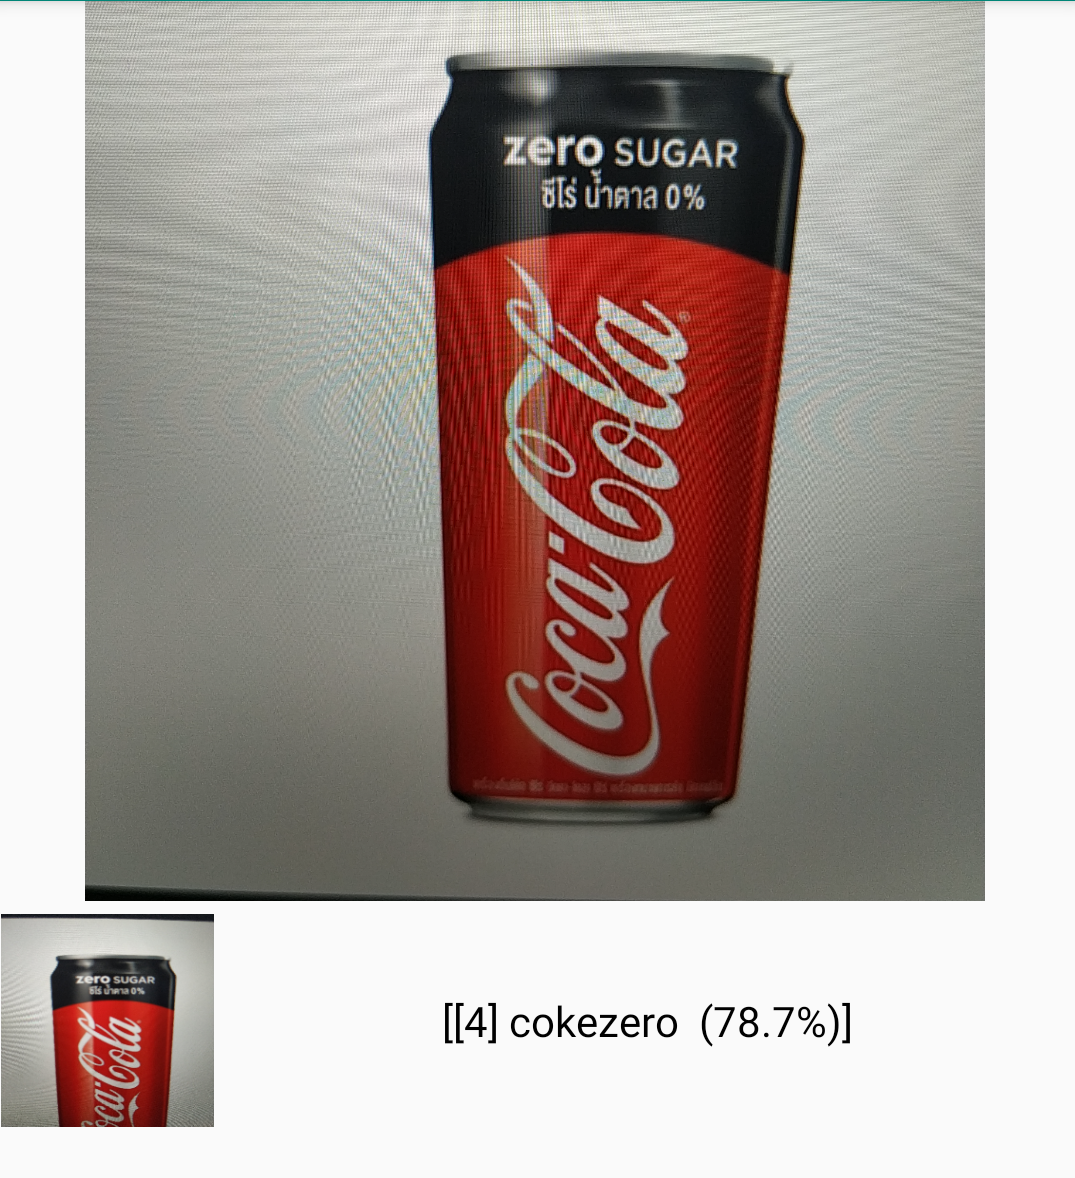
\includegraphics[width=0.4\textwidth]{Figures/5/ze.png}
	\caption{การทดสอบความแม่นยำอาหารชื่อ Cokezero}
	\label{Fig:ze}
\end{figure}
จากรูปที่ \ref{Fig:ze} เป็นรูปผลลัพธ์ของการทำนายอาหารชื่อ Cokezero พบว่ามีค่าความแม่นยำที่ร้อยละ 78
\newpage

\end{itemize}

\begin{itemize}
	\item{การถ่ายภาพอาหารชื่อ Coke}

\begin{figure}[H]
	\centering
	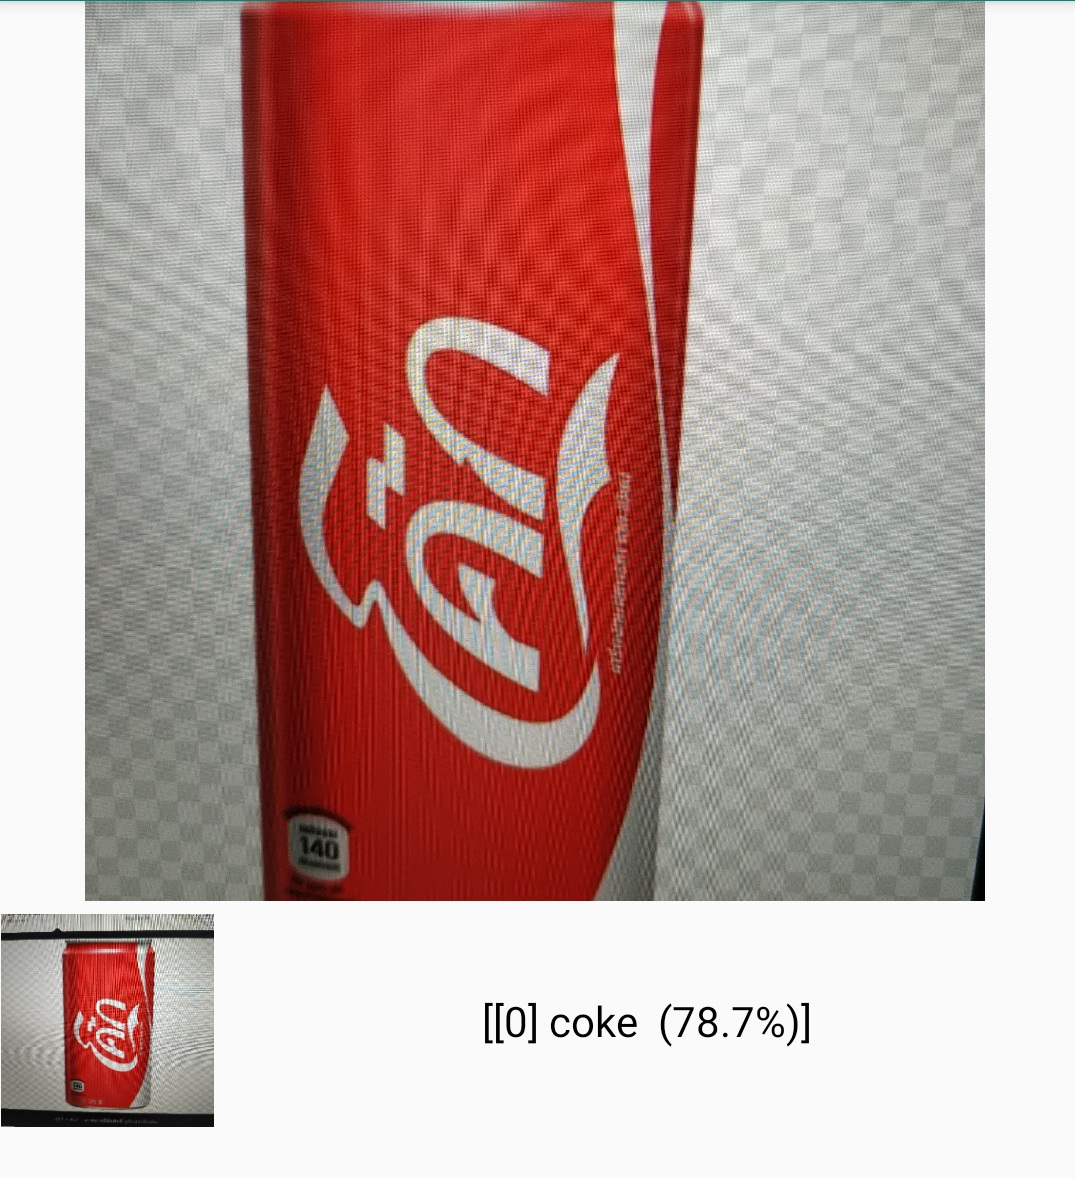
\includegraphics[width=0.4\textwidth]{Figures/5/co.png}
	\caption{การทดสอบความแม่นยำอาหารชื่อ Coke}
	\label{Fig:co}
\end{figure}
จากรูปที่ \ref{Fig:co} เป็นรูปผลลัพธ์ของการทำนายอาหารชื่อ Coke พบว่ามีค่าความแม่นยำที่ร้อยละ 78
\newpage

\end{itemize}


\begin{itemize}
	\item{การถ่ายภาพอาหารชื่อ laysbasilflavor}

\begin{figure}[H]
	\centering
	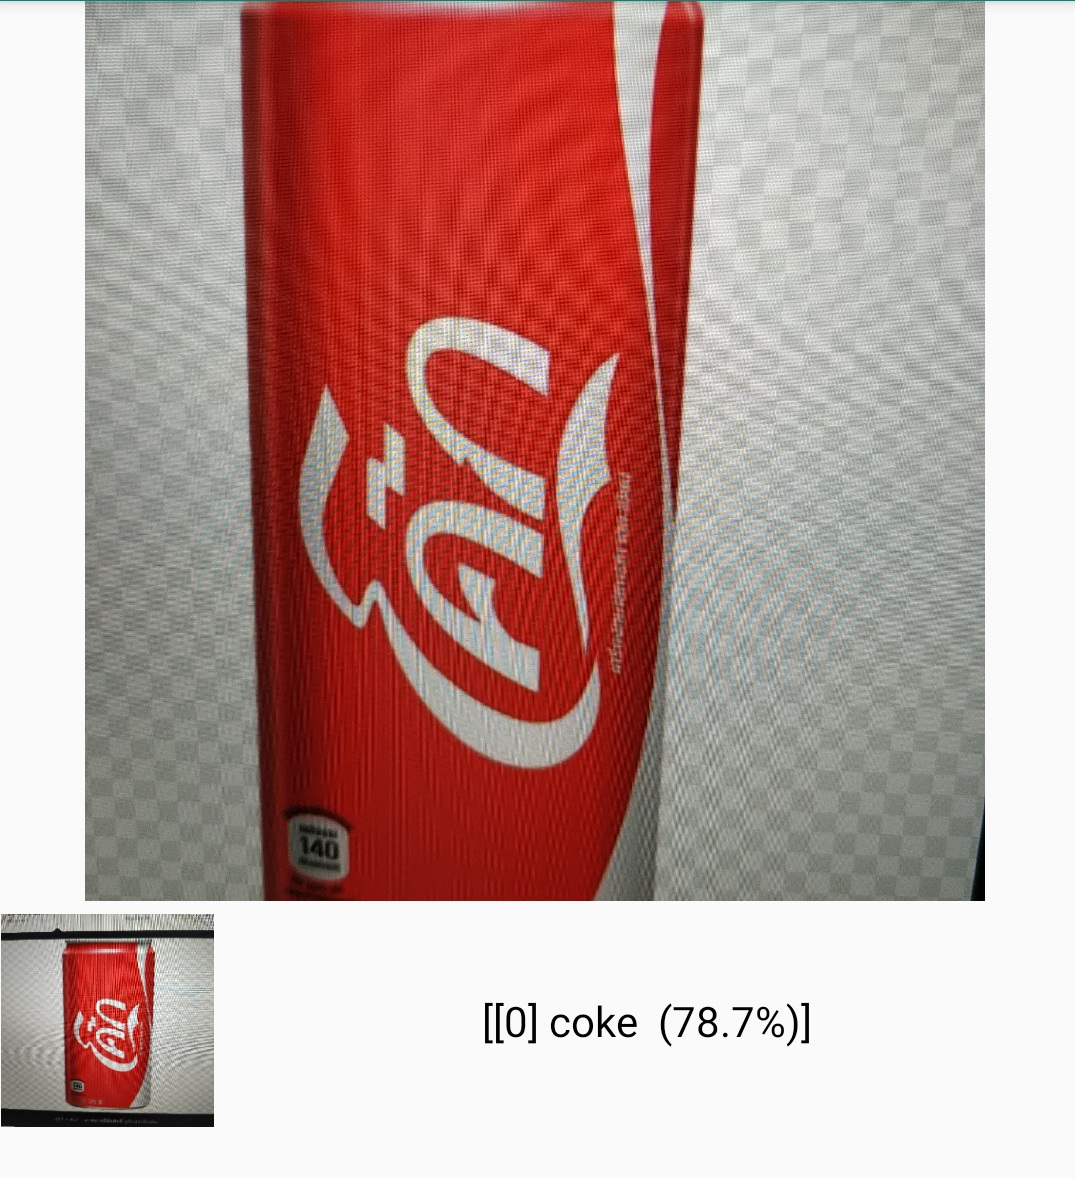
\includegraphics[width=0.4\textwidth]{Figures/5/co.png}
	\caption{การทดสอบความแม่นยำอาหารชื่อ laysbasilflavor}
	\label{Fig:co}
\end{figure}
จากรูปที่ \ref{Fig:co} เป็นรูปผลลัพธ์ของการทำนายอาหารชื่อ laysbasilflavor พบว่ามีค่าความแม่นยำที่ร้อยละ 76
\newpage

\end{itemize}



\begin{itemize}
	\item{การถ่ายภาพอาหารชื่อ bentored}

\begin{figure}[H]
	\centering
	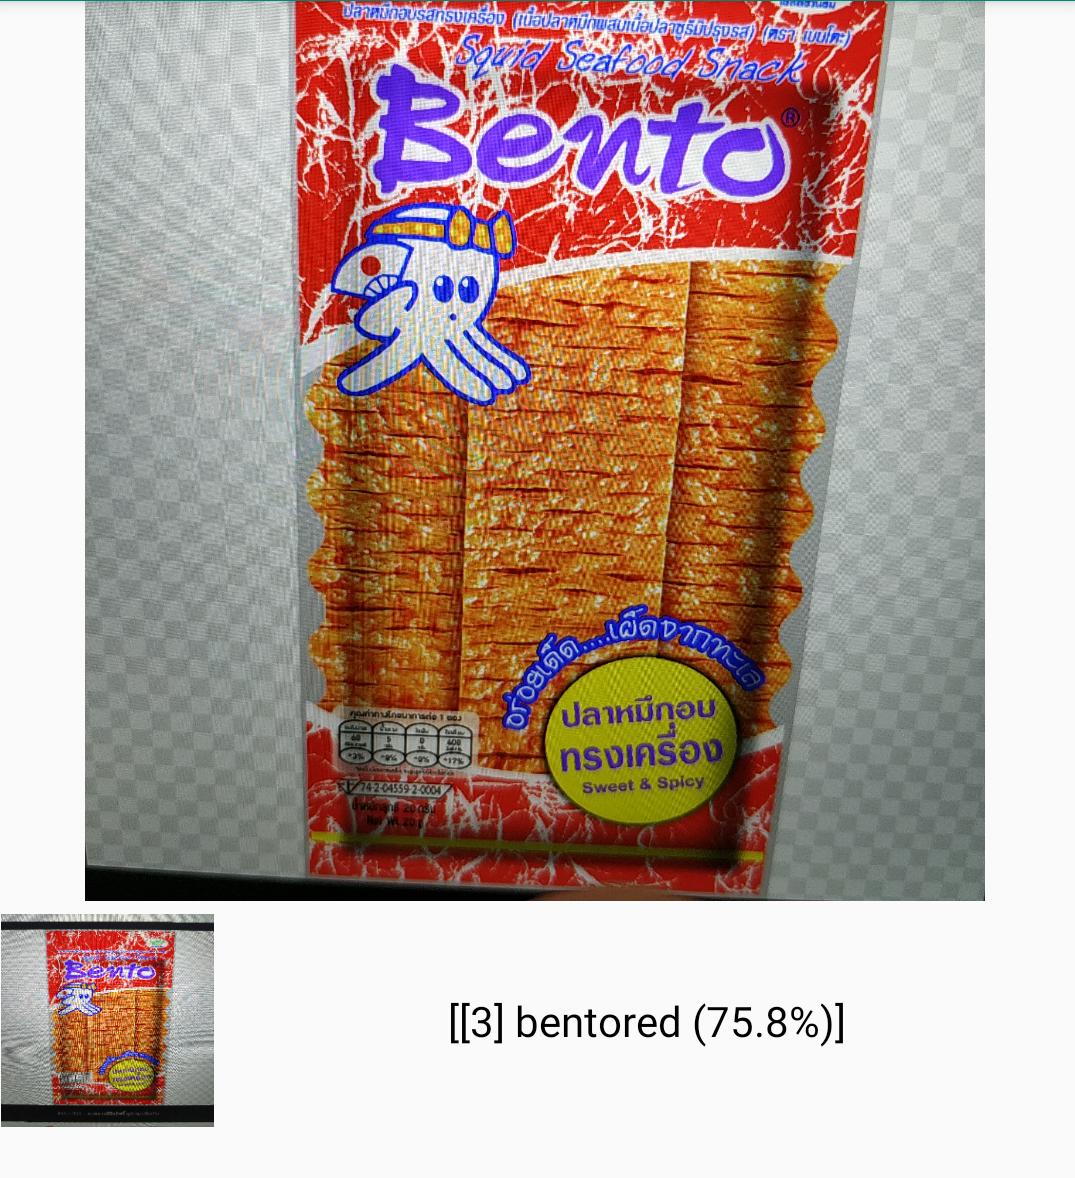
\includegraphics[width=0.4\textwidth]{Figures/5/ben.png}
	\caption{การทดสอบความแม่นยำอาหารชื่อ bentored}
	\label{Fig:bentored}
\end{figure}
จากรูปที่ \ref{Fig:bentored} เป็นรูปผลลัพธ์ของการทำนายอาหารชื่อ bentored พบว่ามีค่าความแม่นยำที่ร้อยละ 75
\newpage

\end{itemize}



\begin{itemize}
	\item{การถ่ายภาพอาหาร hainanesechickenrice}

\begin{figure}[H]
	\centering
	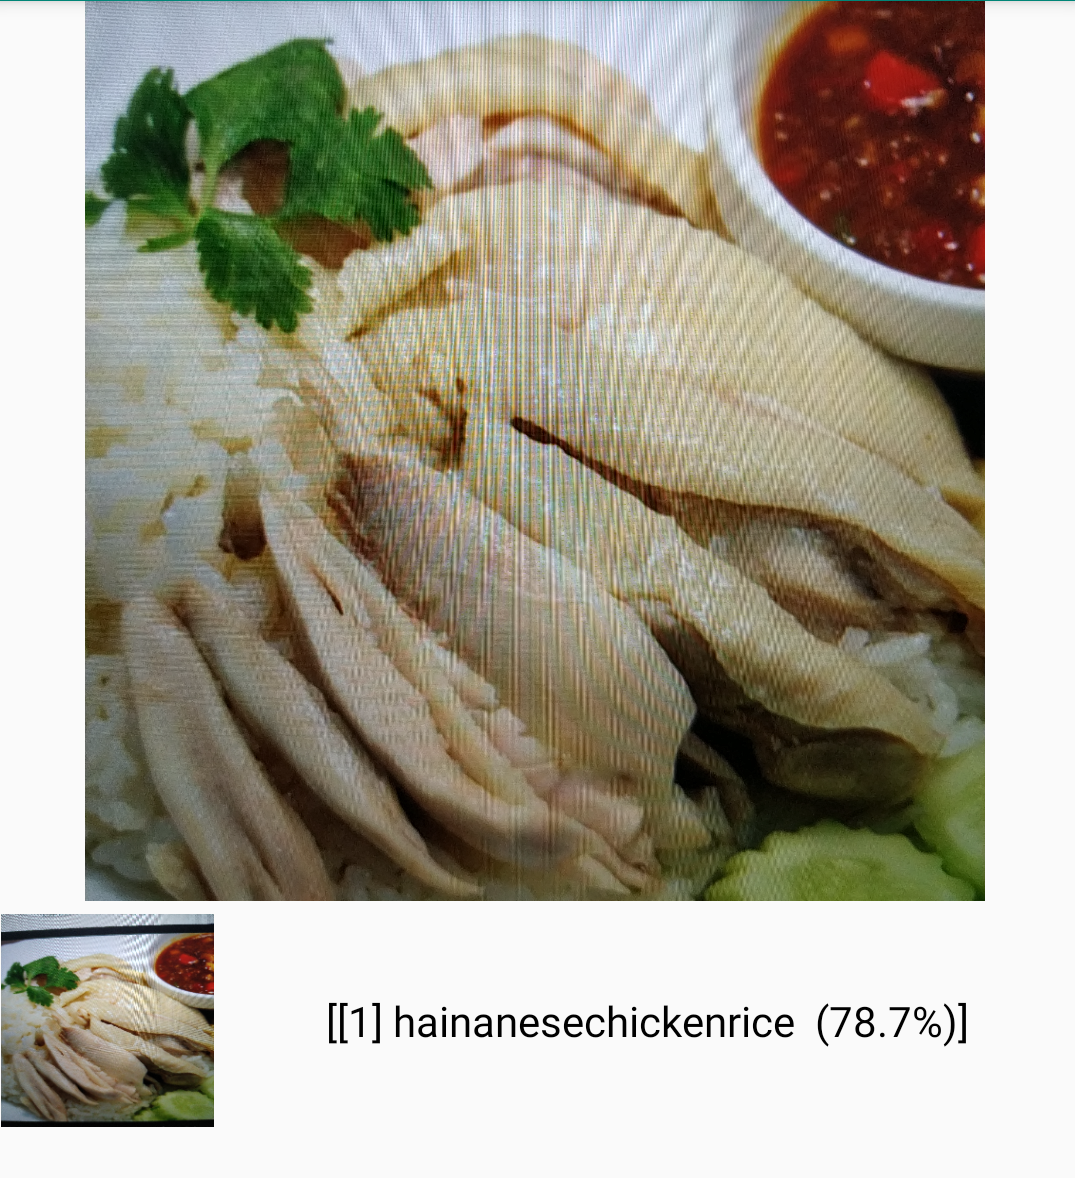
\includegraphics[width=0.4\textwidth]{Figures/5/rice.png}
	\caption{การทดสอบความแม่นยำอาหารชื่อ hainanesechickenrice}
	\label{Fig:rice}
\end{figure}
จากรูปที่ \ref{Fig:rice} เป็นรูปผลลัพธ์ของการทำนายอาหารชื่อ hainanesechickenrice พบว่ามีค่าความแม่นยำ ร้อยละ 78
\newpage

\end{itemize}

\begin{table}[H]
	\caption{ผลการทดสอบความถูกต้องในการทำนาย}
    \label{tab:wrong}
    \centering
	\begin{tabular}{ | p{3cm} | p{3cm} | p{3cm} | p{3cm} | p{3cm} | }
		\hline

		ลำดับ & ชื่ออาหารที่ถ่าย & ผลลัพธ์การทำนาย & ค่าความถูกต้อง  \\ \hline
		\setstretch{1.0}{รูปภาพที่ 1}&\setstretch{1.0}{Cokezero}&\setstretch{1.0}{ถูกต้อง}&\setstretch{1.0}{78\%} \\ \hline
		\setstretch{1.0}{รูปภาพที่ 2}&\setstretch{1.0}{Coke}&\setstretch{1.0}{ถูกต้อง}&\setstretch{1.0}{78\%} \\ \hline
        \setstretch{1.0}{รูปภาพที่ 3}&\setstretch{1.0}{laysbasilflavor}&\setstretch{1.0}{ถูกต้อง}&\setstretch{1.0}{76\%} \\ \hline
        \setstretch{1.0}{รูปภาพที่ 4}&\setstretch{1.0}{ben}&\setstretch{1.0}{ถูกต้อง}&\setstretch{1.0}{75\%}\\ \hline
        \setstretch{1.0}{รูปภาพที่ 5}&\setstretch{1.0}{hainanese chickenrice}&\setstretch{1.0}{ถูกต้อง}&\setstretch{1.0}{78\%} \\ \hline
	\end{tabular}
\end{table} 

จากตารางที่ \ref{tab:wrong}   เป็นค่าคามแม่นยำจากการถ่ายภาพอาหารที่แตกต่างกัน 5 ชนิด โดยมีค่าความแม่นยำมากกว่าร้อยละ 70


